\documentclass[tikz,border=3mm]{standalone}
\usepackage{pgfplots}
\usepgfplotslibrary{groupplots}
\pgfplotsset{compat=1.18}
\definecolor{GridColor}{HTML}{D9E2EF}
\definecolor{mahalanobisColor}{HTML}{2F5597}
\definecolor{mahalanobis_l2Color}{HTML}{5B9BD5}
\definecolor{knnColor}{HTML}{70AD47}
\definecolor{knn_l2Color}{HTML}{FFC000}
\begin{document}
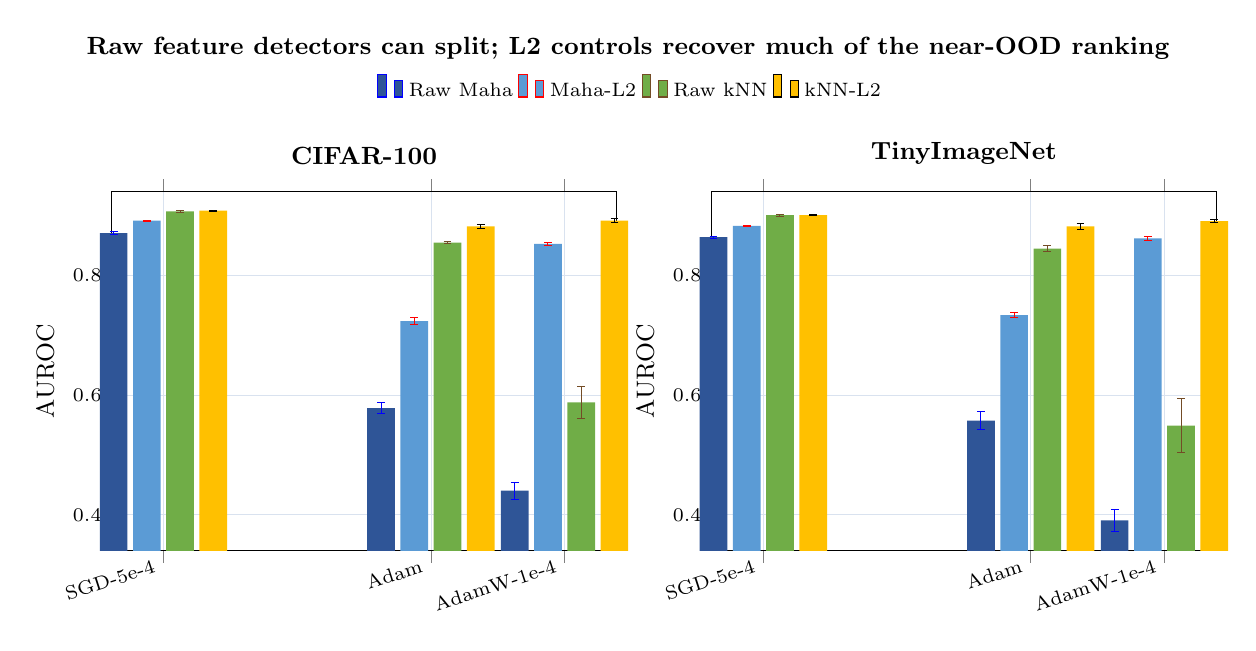
\begin{tikzpicture}
\begin{groupplot}[
  group style={group size=2 by 1,horizontal sep=1.2cm},
  ybar,
  width=8.0cm,
  height=6.15cm,
  ymin=0.34,
  ymax=0.94,
  ylabel={AUROC},
  symbolic x coords={SGD-5e-4,SGD-2e-4,Adam,AdamW-1e-4,AdamW-5e-4},
  xtick=data,
  xticklabel style={font=\scriptsize,rotate=18,anchor=east},
  tick label style={font=\scriptsize},
  label style={font=\small},
  title style={font=\bfseries\small},
  enlarge x limits=0.13,
  grid=major,
  grid style={draw=GridColor,line width=0.25pt},
  legend style={at={(1.03,1.22)},anchor=south,legend columns=4,draw=none,font=\scriptsize},
  error bars/error bar style={line width=0.35pt},
  error bars/error mark options={rotate=90,mark size=1.4pt,line width=0.35pt},
  clip=false
]
\nextgroupplot[title={CIFAR-100}]
\addplot+[fill=mahalanobisColor,draw=none,error bars/.cd,y dir=both,y explicit] coordinates {(SGD-5e-4,0.8700) +- (0,0.0029) (Adam,0.5779) +- (0,0.0087) (AdamW-1e-4,0.4402) +- (0,0.0144)};
\addplot+[fill=mahalanobis_l2Color,draw=none,error bars/.cd,y dir=both,y explicit] coordinates {(SGD-5e-4,0.8905) +- (0,0.0011) (Adam,0.7230) +- (0,0.0057) (AdamW-1e-4,0.8518) +- (0,0.0021)};
\addplot+[fill=knnColor,draw=none,error bars/.cd,y dir=both,y explicit] coordinates {(SGD-5e-4,0.9061) +- (0,0.0010) (Adam,0.8542) +- (0,0.0019) (AdamW-1e-4,0.5875) +- (0,0.0268)};
\addplot+[fill=knn_l2Color,draw=none,error bars/.cd,y dir=both,y explicit] coordinates {(SGD-5e-4,0.9073) +- (0,0.0010) (Adam,0.8810) +- (0,0.0040) (AdamW-1e-4,0.8906) +- (0,0.0033)};
\legend{Raw Maha,Maha-L2,Raw kNN,kNN-L2}
\nextgroupplot[title={TinyImageNet}]
\addplot+[fill=mahalanobisColor,draw=none,error bars/.cd,y dir=both,y explicit] coordinates {(SGD-5e-4,0.8631) +- (0,0.0016) (Adam,0.5572) +- (0,0.0143) (AdamW-1e-4,0.3909) +- (0,0.0185)};
\addplot+[fill=mahalanobis_l2Color,draw=none,error bars/.cd,y dir=both,y explicit] coordinates {(SGD-5e-4,0.8818) +- (0,0.0005) (Adam,0.7329) +- (0,0.0044) (AdamW-1e-4,0.8610) +- (0,0.0029)};
\addplot+[fill=knnColor,draw=none,error bars/.cd,y dir=both,y explicit] coordinates {(SGD-5e-4,0.8997) +- (0,0.0013) (Adam,0.8441) +- (0,0.0055) (AdamW-1e-4,0.5486) +- (0,0.0447)};
\addplot+[fill=knn_l2Color,draw=none,error bars/.cd,y dir=both,y explicit] coordinates {(SGD-5e-4,0.8997) +- (0,0.0010) (Adam,0.8811) +- (0,0.0053) (AdamW-1e-4,0.8899) +- (0,0.0030)};
\end{groupplot}
\node[anchor=south,font=\bfseries\small] at (current bounding box.north)
{Raw feature detectors can split; L2 controls recover much of the near-OOD ranking};
\end{tikzpicture}
\end{document}
